\section{System architecture}\label{sec:architecture}
The system separates scientific computation from evidence presentation.
Figure~\ref{fig:architecture} shows the implemented flow: an original physical
model enters a native numerical method, its output is evaluated independently,
and a versioned export is consumed by a static reader. The reader does not
compute a new optimizer by displaying an existing result. This separation
keeps numerical source identity, local user execution and web distribution
independently inspectable. A successful web build establishes neither the
installability of a native wheel nor the scientific acceptance of every
numerical result referenced by that build.
\begin{figure}[htbp]\centering
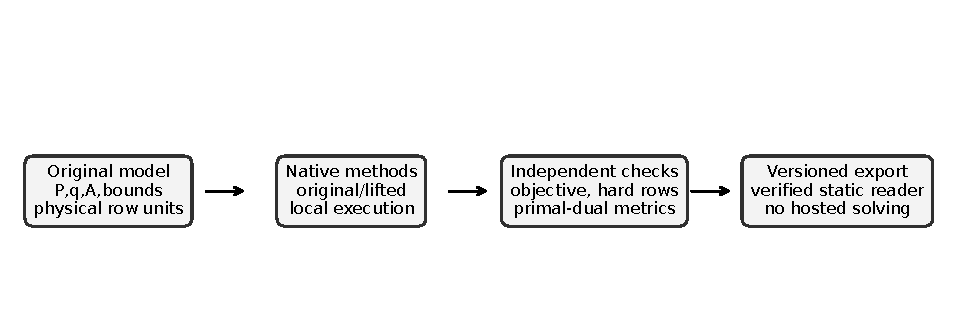
\includegraphics[width=.94\textwidth]{figures/architecture.pdf}
\caption{Implemented data flow from original physical model through native solving and independent acceptance to a versioned static reader. This is an architecture diagram, not a measured speed or reliability result.}\label{fig:architecture}
\end{figure}


The first processing stage constructs or ingests a canonical original-space
problem and physical row descriptions. Authored scalar and control cases
come from deterministic generators. The source-faithful building adapter
preserves its upstream mixed penalties, while separate constructors identify
authored policy variants. Structural validation checks sparse dimensions,
finite numeric values, interval order, units and hard/soft policy before a
backend is selected. Native method packages are owned by a separate public
engine repository; the product scripts do not hide an unpublished internal
solver distribution.

The method stage applies an explicit compatibility rule and runs an admitted
objective using fixed settings. It records available, incompatible and failed
outcomes with reasons. Prepared workspaces retain only the structure their
interface permits, including matrix patterns, coefficients and hard masks.
The evaluation stage recovers original coordinates, objective components,
lower/upper departures and hard error; grouped repeated operations additionally
retain framewise primal and dual checks. This order prevents a library success
flag from being exported as scientific acceptance before original quantities
have been checked.

The export stage validates the scientific documents against their schemas,
writes exact finite UTF-8 data, and produces checksummed inventories and
deployment manifests. Readiness is calculated from actual files and contract
states. JSONL preserves nested diagnostics and unsuccessful observations;
CSV provides a projection for inspection. The static frontend verifies byte
identities and schema/cross-field constraints before rendering a selected case
or an experimental comparison. Its unit filter avoids combining physically
incommensurable departures in one raw numerical axis.

The local cost editor creates a bounded request against a canonical digest.
The user explicitly runs the native scientific command outside the browser
and imports its result envelope. The reader checks that the request, model,
prices, hard policy and recovered metrics agree. Canonical replay and local
native imports receive different provenance labels. A selected C12 stream
cannot be reused after a local policy edit because its stored inputs no
longer match the edited model. The optional API remains a dormant file-serving
component rather than an optimization endpoint.

The grouped research and teaching profiles are separate from the ordinary
public-SDK profile. Their batches, observations and split summaries have
schemas and complete external evidence, but no installed browser replay
adapter. The teaching worker uses direct external CPython, a public SDK
fingerprint and bounded process cleanup. These boundaries permit actual
native methods to be taught without claiming that their external execution
has become a browser capability. No training or fitted model stage exists:
the implemented methods are deterministic optimization procedures, and the
unavailable learned FlexQP policy is not replaced by a fabricated checkpoint.

The distributed application has six scientific routes, but route count is
not a proxy for numerical depth. Scientific authority resides in the exact
inputs, implementations, protocols and accepted outputs. The deployment
workflow builds committed evidence and checks its own commit identity; it
does not regenerate an experimental study to refresh a version badge. This
architecture enables reproducible inspection while retaining the limits of
synthetic data and externally executed numerical work.
